\documentclass[a4paper,11pt]{article}

\usepackage[T1]{fontenc}
\usepackage[utf8]{inputenc}
\usepackage[english]{babel}
\usepackage[top=2.5cm, bottom=2.5cm, left=2.5cm, right=2.5cm]{geometry}
\usepackage{listings}
\usepackage{xcolor}
\usepackage{microtype}
\usepackage{booktabs}
\usepackage{tabularx}
\usepackage{enumitem}
\usepackage{hyperref}
\usepackage{amsmath}
\usepackage{amssymb}
\usepackage{tikz}
\usepackage{caption}
\usepackage{abstract}
\usepackage{titlesec}
\usepackage{parskip}
\usepackage{graphicx}
\usepackage{float}

\usetikzlibrary{positioning,calc,decorations.pathreplacing}

\usepackage{mathptmx}   % Times-compatible serif (~ Liberation Serif)
\usepackage{helvet}     % Helvetica-compatible sans (~ Liberation Sans)
\usepackage{courier}    % monospace (~ DejaVu Sans Mono)

% Colors
\definecolor{codebg}{RGB}{244,248,240}
\definecolor{codegreen}{RGB}{26,85,26}
\definecolor{headcolor}{RGB}{46,64,87}
\definecolor{sectioncolor}{RGB}{26,107,138}
\definecolor{keywordcolor}{RGB}{0,70,140}
\definecolor{commentcolor}{RGB}{100,100,100}
\definecolor{stringcolor}{RGB}{150,0,0}
\definecolor{boxblue}{RGB}{208,225,242}
\definecolor{boxgreen}{RGB}{214,234,214}
\definecolor{boxyellow}{RGB}{252,243,207}

% Captions in the small-italic style used by the Selfie theses
\captionsetup{font={small,it}, labelfont={small,it}}

% Hyperref setup
\hypersetup{
  colorlinks=true,
  linkcolor=sectioncolor,
  citecolor=sectioncolor,
  urlcolor=sectioncolor,
}

% C* with the auto keyword
\lstdefinelanguage{Cstar}{
  keywords={auto, if, else, while, return, void, uint64_t, char, malloc, sizeof},
  keywordstyle=\bfseries\color{keywordcolor},
  comment=[l]{//},
  commentstyle=\itshape\color{commentcolor},
  stringstyle=\color{stringcolor},
  morestring=[b]",
  sensitive=true
}

\lstset{
  language=Cstar,
  backgroundcolor=\color{codebg},
  basicstyle=\ttfamily\small,
  frame=single,
  framerule=0.4pt,
  rulecolor=\color{lightgray},
  xleftmargin=10pt,
  xrightmargin=10pt,
  framexleftmargin=6pt,
  framexrightmargin=6pt,
  framextopmargin=4pt,
  framexbottommargin=4pt,
  breaklines=true,
  showstringspaces=false,
  tabsize=4,
  aboveskip=6pt,
  belowskip=6pt,
  numbers=left,
  numberstyle=\tiny\color{gray},
  numbersep=6pt,
}

% A plain "Code block" pseudocode style (no line numbers, no language)
\lstdefinestyle{pseudocode}{
  language={},
  backgroundcolor=\color{white},
  basicstyle=\ttfamily\small,
  numbers=none,
  keywordstyle=\bfseries,
  morekeywords={IF,ELSE,WHILE,RETURN,return},
  frame=single,
  framerule=0.4pt,
  rulecolor=\color{black},
}

\titleformat{\section}{\large\bfseries\color{headcolor}}{{\thesection}}{1em}{}[\vspace{-4pt}\rule{\textwidth}{0.4pt}]
\titleformat{\subsection}{\normalsize\bfseries\color{sectioncolor}}{\thesubsection}{1em}{}
\titleformat{\subsubsection}{\small\bfseries\color{sectioncolor}}{\thesubsubsection}{1em}{}

\setlength{\parskip}{6pt}
\setlength{\parindent}{0pt}

\begin{document}

% ── Title ─────────────────────────────────────────────────────────────────────
\begin{center}
  {\LARGE \textbf{\textcolor{headcolor}{\texttt{auto}: Initialiser-Driven Type Deduction in Selfie}}}\\[0.4cm]
  {\large Adding type inference to a single-pass C* compiler without an AST}\\[0.6cm]
  {\normalsize
    Florian Schroffner\\
    \texttt{florian.schroffner@stud.plus.ac.at}\\
    Department of Computer Sciences, University of Salzburg\\
    Advanced Systems Engineering\\
    Supervisor: Univ.-Prof.\ Dr.\ Christoph Kirsch\\[0.2cm]
    \today
  }
\end{center}

\vspace{0.3cm}
\hrule height 1pt
\vspace{0.5cm}

% ── Abstract ──────────────────────────────────────────────────────────────────
\begin{abstract}
\noindent
This work extends the Selfie/C* compiler with a single keyword, \texttt{auto}, that gives a local variable the type of its initialiser. The feature is added \emph{without} changing Selfie's single-pass architecture: no abstract syntax tree (AST), no separate semantic pass, and no change to the code generator. The enabling observation is that Selfie's parser already performs lightweight type tracking --- every expression-compiling function \emph{returns} the type (\texttt{uint64\_t} or \texttt{uint64\_t*}) of the value it just emitted --- so the type an \texttt{auto} variable needs is already computed the moment its initialiser is parsed. We distinguish the mechanism we add, \emph{type deduction} (local, one-directional, as in C++ and Go), from full \emph{type inference} (global, constraint-solving, as in the ML family), and argue that it is precisely deduction's locality that makes it fit a single pass. The implementation touches three functions in \texttt{selfie.c} plus a one-keyword scanner addition. The extended compiler still self-compiles to a 43\,624-instruction RISC-U binary and passes the project autograder, including a dedicated \texttt{auto}-type-inference suite. As a self-application test, 79 of \texttt{selfie.c}'s own local declarations are rewritten cast-free to \texttt{auto}; the compiler translates this version of itself and still reaches a self-self fixpoint. We conclude that a feature usually associated with multi-pass compilers does not, in its initialiser-driven form, require multi-pass machinery.

\vspace{4pt}
\noindent\textbf{Keywords:} Type Deduction, Type Inference, \texttt{auto}, Single-Pass Compiler, Recursive-Descent Parsing, Selfie, C*, RISC-U, Self-Compilation
\end{abstract}

\hrule height 0.4pt
\vspace{0.3cm}

% ══════════════════════════════════════════════════════════════════════════════
\section{Introduction}
\label{sec:introduction}

\subsection{Problem Definition}
\label{sec:problem}

In C and most C-family languages every local variable is declared with an explicit type, even when that type is obvious from the value it is initialised with. Modern languages remove this redundancy: C++ offers \texttt{auto}, Go provides \texttt{:=}, and the ML family infers types across whole functions. A common assumption is that adding such a feature to a compiler requires a multi-pass pipeline with an explicit AST and a dedicated semantic phase that can reason about types before code generation. Selfie's compiler has neither: it is single-pass and emits machine code as it parses. The problem this work addresses is therefore whether type inference can be added to Selfie \emph{without} abandoning its defining single-pass, AST-free design.

\subsection{Contribution}
\label{sec:contribution}

We design and implement the \texttt{auto} keyword for local variables in C*, the language compiled by Selfie. A variable declared \texttt{auto} takes the type of its initialiser. The feature is realised entirely within Selfie's single pass by reading back type information the parser already produces, so it adds no AST and no separate pass. We touch three functions in \texttt{selfie.c}. The extended compiler still self-compiles and passes the autograder. In addition, we dogfood the feature on the compiler itself: 79 of \texttt{selfie.c}'s own local declarations are folded into \texttt{auto} cast-free, and the resulting compiler still reaches a self-self fixpoint. Finally, we analyse why the mechanism is cheap by separating \emph{type deduction} from \emph{type inference}, and we relate the feature's restrictions to the boundary of what a single pass makes available.

This work answers three research questions:

\begin{enumerate}[leftmargin=*, label=\textbf{RQ\arabic*.}]
  \item Can initialiser-driven \texttt{auto} deduction be added to a single-pass compiler without introducing an AST or a separate semantic pass?
  \item What is the smallest set of changes to \texttt{selfie.c} that implements \texttt{auto} correctly, including stack allocation and procedure cleanup?
  \item Does the resulting compiler still satisfy Selfie's self-referentiality requirement --- that it compile its own source --- even when that source itself uses \texttt{auto}?
\end{enumerate}

\subsection{Type Inference Primer}
\label{sec:primer}

\subsubsection{Type Deduction versus Type Inference}
\label{sec:deduction-vs-inference}

The phrase ``type inference'' is used loosely for two mechanisms that differ sharply in cost and power. Telling them apart is essential to understanding what this work does --- and what it deliberately does not.

\textbf{Type deduction (local, one-directional).} Given a variable whose initialiser is a \emph{fully typed} expression, the variable simply adopts that expression's type. Information flows in one direction only --- from the right-hand side of the \texttt{=} to the variable on the left --- and there is nothing to \emph{solve}: the type of the initialiser is already known the moment the declaration is read. This is what C++ does --- the ISO standard literally calls it ``\texttt{auto} type \emph{deduction}'' \cite{cppstd} --- what Go's \texttt{:=} does, and what C23 \texttt{auto} \cite{c23} performs. A deducer never reasons about how the variable is \emph{used} afterwards; it inspects only the single expression to its right.

\textbf{Type inference (global, bidirectional).} Languages of the ML family --- Haskell, OCaml, Standard ML --- assign types to variables and functions that carry \emph{no} annotation on either side. They do so by collecting \emph{constraints} from every use across a definition (or the whole program) and \emph{solving} them by unification, the Hindley--Milner algorithm~\cite{hindleymilner}. Type information may flow \emph{backward}, from a later use to an earlier definition, and a value may be \emph{generalised} to a polymorphic type. In \texttt{let n = read () in n + 1}, an inferrer can fix the type of \texttt{n} from the way it is later used; a deducer cannot, because it has already moved past the declaration.

\textbf{Why the distinction is architectural.} Hindley--Milner inference needs a structure that survives long enough to gather constraints from many program points --- in practice an AST and a separate solving pass. Deduction needs neither: the one expression to the right of \texttt{=} is sufficient, and it can be consumed the instant it is parsed. \emph{What this work adds to Selfie is type deduction, not Hindley--Milner inference}, and that is exactly why it fits a single pass with no AST. We keep the customary word ``inference'' in the keyword's informal name (as C++ programmers colloquially do), but the mechanism is deduction; Section~\ref{sec:implementation} makes its one-directional, initialiser-only nature explicit.

\subsection{The Target Architecture}
\label{sec:architecture}

Although deduction needs no knowledge of the target machine, the implementation does: an \texttt{auto} declaration must reserve storage for its variable, and in Selfie that storage lives on the call stack. This section reviews the parts of Selfie's target needed to follow the implementation.

\subsubsection{RISC-U and C*}
\label{sec:riscu}

Selfie~\cite{selfie} compiles C* to RISC-U. C* is a strict subset of C with only two types --- the unsigned 64-bit integer \texttt{uint64\_t} and the pointer \texttt{uint64\_t*} --- no floating point, and no composite types. RISC-U is a tiny subset of the RISC-V instruction set with 14 instructions (\texttt{lui}, \texttt{addi}, \texttt{add}, \texttt{sub}, \texttt{mul}, \texttt{divu}, \texttt{remu}, \texttt{sltu}, \texttt{ld}, \texttt{sd}, \texttt{beq}, \texttt{jal}, \texttt{jalr}, \texttt{ecall}). Because both registers and datatypes are 64-bit, a valid address is always a multiple of eight bytes. The two-type system is central to this work: it is why \texttt{auto} has only two possible answers and why there is no promotion lattice to search.

\subsubsection{Memory}
\label{sec:memory}

A RISC-U program runs in a byte-addressed linear address space divided into four segments: code, data, heap, and stack (Figure~\ref{fig:memory}). Code and data are static and fixed at compile time; the heap and stack are dynamic. The heap sits just above the static data and grows upward (it backs \texttt{malloc}); the stack sits at the top of memory and grows downward. The boundary between the static and dynamic parts is the program break (Equation~\ref{eq:break}).

\begin{figure}[H]
\centering
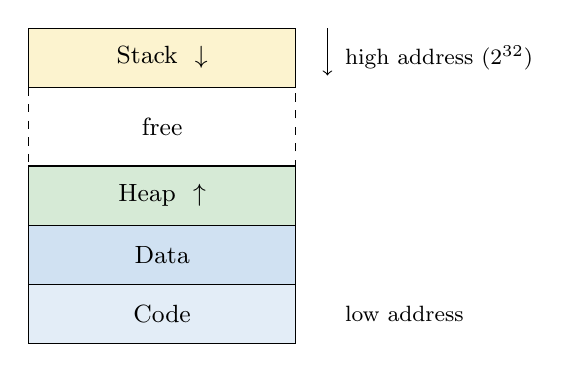
\begin{tikzpicture}[every node/.style={font=\small}]
  \tikzstyle{seg}=[draw, minimum width=3.4cm, minimum height=0.75cm, outer sep=0pt]
  \node[seg, fill=boxyellow] (stack) {Stack \ $\downarrow$};
  \node[seg, dashed, below=0pt of stack, minimum height=1.0cm] (free) {free};
  \node[seg, fill=boxgreen, below=0pt of free] (heap) {Heap \ $\uparrow$};
  \node[seg, fill=boxblue, below=0pt of heap] (data) {Data};
  \node[seg, fill=boxblue!60, below=0pt of data] (code) {Code};
  \draw[->] ($(stack.north east)+(0.4,0)$) ++(0,0) -- ++(0,-0.6) node[midway,right]{};
  \node[right=0.5cm of stack, font=\footnotesize] {high address ($2^{32}$)};
  \node[right=0.5cm of code, font=\footnotesize] {low address};
\end{tikzpicture}
\caption{Memory segment order. Code and data are static; heap and stack are dynamic and grow towards each other.}
\label{fig:memory}
\end{figure}

\begin{equation}
\textit{program\_break} = 65536 + \textit{code\_segment\_size} + \textit{data\_segment\_size}
\label{eq:break}
\end{equation}
\vspace{-12pt}
\begin{center}\small\itshape Equation 1: program break\end{center}

\subsubsection{Function Calling Convention and the Stack Frame}
\label{sec:frame}

Local variables live in the call stack. On a call, the caller pushes any live temporaries and the arguments; the callee's prologue then saves the return address and the caller's frame pointer, sets up its own frame pointer in register \texttt{S0}, and reserves space for the callee's local variables by lowering the stack pointer \texttt{SP}. Locals are addressed at negative offsets from the frame pointer. Figure~\ref{fig:frame} shows the layout; the shaded region marks the contribution \texttt{auto} adds, explained in Section~\ref{sec:lazy}.

\begin{figure}[H]
\centering
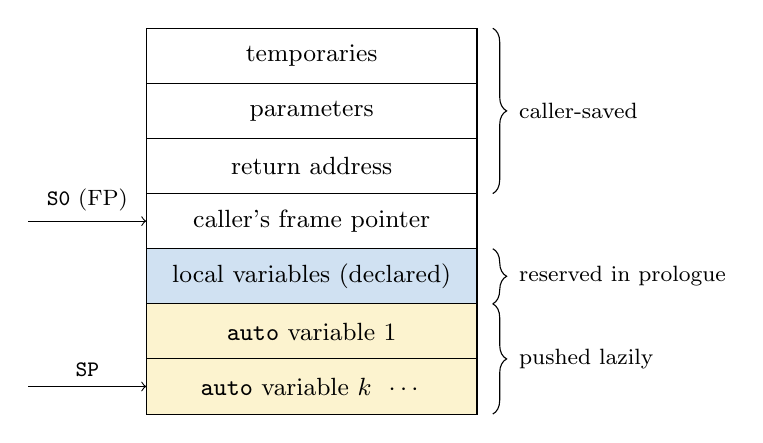
\begin{tikzpicture}[every node/.style={font=\small}]
  \tikzstyle{slot}=[draw, minimum width=4.2cm, minimum height=0.7cm, outer sep=0pt]
  \node[slot] (temp) {temporaries};
  \node[slot, below=0pt of temp] (param) {parameters};
  \node[slot, below=0pt of param] (ra) {return address};
  \node[slot, below=0pt of ra] (fp) {caller's frame pointer};
  \node[slot, fill=boxblue, below=0pt of fp] (locals) {local variables (declared)};
  \node[slot, fill=boxyellow, below=0pt of locals, minimum height=0.7cm] (auto1) {\texttt{auto} variable $1$};
  \node[slot, fill=boxyellow, below=0pt of auto1] (auto2) {\texttt{auto} variable $k$ \ $\cdots$};
  % FP and SP markers
  \draw[->] ($(fp.west)+(-1.5,0)$) -- (fp.west) node[midway,above,font=\footnotesize]{\texttt{S0} (FP)};
  \draw[->] ($(auto2.west)+(-1.5,0)$) -- (auto2.west) node[midway,above,font=\footnotesize]{\texttt{SP}};
  % braces
  \draw[decorate, decoration={brace, amplitude=5pt}] ($(temp.north east)+(0.2,0)$) -- ($(ra.south east)+(0.2,0)$) node[midway, right=6pt, font=\footnotesize]{caller-saved};
  \draw[decorate, decoration={brace, amplitude=5pt}] ($(locals.north east)+(0.2,0)$) -- ($(locals.south east)+(0.2,0)$) node[midway, right=6pt, font=\footnotesize]{reserved in prologue};
  \draw[decorate, decoration={brace, amplitude=5pt}] ($(auto1.north east)+(0.2,0)$) -- ($(auto2.south east)+(0.2,0)$) node[midway, right=6pt, font=\footnotesize]{pushed lazily};
\end{tikzpicture}
\caption{Call stack frame. Declared locals are reserved once in the prologue; each \texttt{auto} variable pushes its own word below them, lazily, as it is compiled.}
\label{fig:frame}
\end{figure}

\subsubsection{The Single-Pass Compiler}
\label{sec:singlepass}

Selfie's compiler is a single-pass recursive-descent parser: scanner, parser, and code emitter advance in lock-step (Figure~\ref{fig:pipeline}). As tokens are consumed, RISC-U code is emitted immediately. There is no explicit AST; the syntax ``tree'' exists only implicitly in the call stack of the parser. The key property this work exploits is that the expression-compiling functions \emph{return a type tag}. As \texttt{compile\_expression()} and the precedence levels below it (\texttt{compile\_arithmetic()}, \texttt{compile\_term()}, \texttt{compile\_factor()}) emit code that computes a value into a temporary register, each returns the type (\texttt{UINT64\_T} or \texttt{UINT64STAR\_T}) of that value (Figure~\ref{fig:typeflow}).

\begin{figure}[H]
\centering
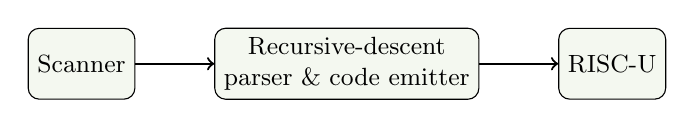
\begin{tikzpicture}[every node/.style={font=\small}, node distance=0.7cm]
  \tikzstyle{stage}=[draw, rounded corners, minimum height=0.9cm, align=center, fill=codebg]
  \node[stage] (sc) {Scanner};
  \node[stage, right=1.0cm of sc] (pa) {Recursive-descent\\parser \& code emitter};
  \node[stage, right=1.0cm of pa] (ru) {RISC-U};
  \draw[->, thick] (sc) -- (pa);
  \draw[->, thick] (pa) -- (ru);
\end{tikzpicture}
\caption{Selfie's single pass: scanner, parser, and emitter advance in lock-step, producing RISC-U directly with no intermediate AST.}
\label{fig:pipeline}
\end{figure}

\begin{figure}[H]
\centering
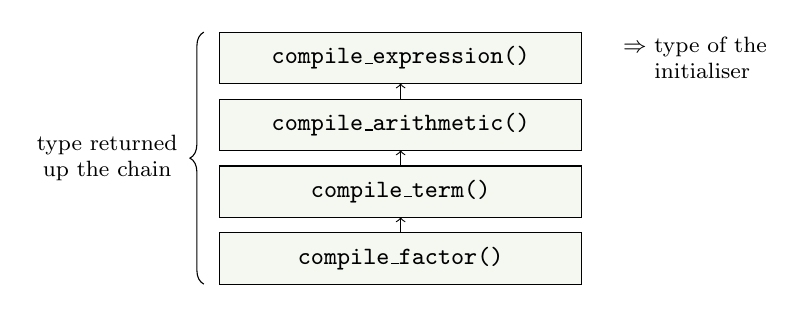
\begin{tikzpicture}[every node/.style={font=\small}]
  \tikzstyle{fn}=[draw, minimum width=4.6cm, minimum height=0.65cm, outer sep=0pt, fill=codebg]
  \node[fn] (expr) {\texttt{compile\_expression()}};
  \node[fn, below=0.2cm of expr] (arith) {\texttt{compile\_arithmetic()}};
  \node[fn, below=0.2cm of arith] (term) {\texttt{compile\_term()}};
  \node[fn, below=0.2cm of term] (factor) {\texttt{compile\_factor()}};
  \draw[->] (factor) -- (term);
  \draw[->] (term) -- (arith);
  \draw[->] (arith) -- (expr);
  \draw[decorate, decoration={brace, amplitude=5pt}] ($(factor.south west)+(-0.2,0)$) -- ($(expr.north west)+(-0.2,0)$) node[midway, left=6pt, font=\footnotesize, align=center]{type returned\\up the chain};
  \node[right=0.4cm of expr, font=\footnotesize, align=left] {$\Rightarrow$ type of the\\\phantom{$\Rightarrow$} initialiser};
\end{tikzpicture}
\caption{Each precedence level returns the type tag of the value it compiled. The type \texttt{auto} needs is the return value of \texttt{compile\_expression()}.}
\label{fig:typeflow}
\end{figure}

\subsubsection{Availability}
\label{sec:availability}

This architecture is implemented by the Selfie project~\cite{selfie}, an educational platform for teaching the design and implementation of compilers, emulators, and hypervisors. Selfie is a single self-compiling file of roughly 12\,000 lines. The design of its compiler is inspired by the Oberon compiler of Niklaus Wirth~\cite{wirth}. Several features have been added to Selfie as bachelor projects in this same single-pass spirit, for instance a conservative garbage collector~\cite{bachinger}; the present work follows that tradition.

% ══════════════════════════════════════════════════════════════════════════════
\section{The \texttt{auto} Implementation}
\label{sec:implementation}

This section describes the actual implementation. As with the rest of Selfie, the goal is to keep it as small as possible: \texttt{auto} is realised by reusing existing machinery rather than adding new subsystems.

\subsection{The Interface}
\label{sec:interface}

To the C* programmer, \texttt{auto} is a drop-in for a type in a local declaration with an initialiser. The extension keeps C* a strict superset: every valid C* program still compiles unchanged, and no new type keyword is introduced. An \texttt{auto} declaration is an ordinary statement inside any procedure body, including \texttt{main} (Listing~\ref{lst:example}).

\begin{lstlisting}[caption={A complete program using \texttt{auto}}, label={lst:example}]
uint64_t factorial(uint64_t n) {
    if (n == 0) return 1;
    return n * factorial(n - 1);
}

uint64_t main() {
    auto n   = 5;             // uint64_t
    auto res = factorial(n);  // uint64_t  -- callee return type
    auto p   = malloc(8);     // uint64_t* -- malloc result
    *p = res;
    auto v   = *p;            // uint64_t  -- dereference
    return v - 120;           // 0 on success
}
\end{lstlisting}

\subsection{Scanner: the \texttt{SYM\_AUTO} Symbol}
\label{sec:scanner}

The scanner gains a single keyword. The identifier \texttt{auto} is recognised and mapped to a new symbol \texttt{SYM\_AUTO}, exactly as the existing type keywords map to \texttt{SYM\_UINT64}. This is the only change to the scanner.

\subsection{The Two Deducible Types}
\label{sec:types}

\texttt{auto} deduces one of Selfie's two existing types (Table~\ref{tab:types}). It adds no types, widths, or conversions: the deduced type is precisely what Selfie's expression compiler already produces for the initialiser. Because there is no second numeric type, there is no promotion rule and no implicit conversion to specify. The pointer rules are inherited verbatim from C* (Table~\ref{tab:ptrs}); \texttt{auto} merely reports their result.

\begin{table}[H]
\centering
\caption{The two types \texttt{auto} can deduce}
\label{tab:types}
\begin{tabular}{llll}
\toprule
\textbf{Type} & \textbf{Internal tag} & \textbf{Example} & \textbf{Deduced Type} \\
\midrule
\texttt{uint64\_t}  & \texttt{UINT64\_T}     & \texttt{auto y = 1;}          & \texttt{uint64\_t}  \\
\texttt{uint64\_t*} & \texttt{UINT64STAR\_T} & \texttt{auto p = malloc(8);}  & \texttt{uint64\_t*} \\
\bottomrule
\end{tabular}
\end{table}

\begin{table}[H]
\centering
\caption{Pointer type rules (unchanged from Selfie)}
\label{tab:ptrs}
\begin{tabular}{lll}
\toprule
\textbf{Expression}        & \textbf{Condition}                                & \textbf{Result Type} \\
\midrule
\texttt{auto v = *p}       & \texttt{p : uint64\_t*}                           & \texttt{uint64\_t}   \\
\texttt{auto q = p + n}    & \texttt{p : uint64\_t*}, \texttt{n : uint64\_t}   & \texttt{uint64\_t*}  \\
\texttt{auto d = p - q}    & \texttt{p, q : uint64\_t*}                        & \texttt{uint64\_t}   \\
\texttt{auto r = malloc(n)}& \texttt{n : uint64\_t}                            & \texttt{uint64\_t*}  \\
\texttt{p + q}             & \texttt{p, q : uint64\_t*}                        & \textbf{Error}       \\
\bottomrule
\end{tabular}
\end{table}

\subsection{Parsing an \texttt{auto} Declaration}
\label{sec:parse}

The core of the feature is the new function \texttt{compile\_auto\_declaration()}. At a high level it parses \texttt{auto identifier = expression ;}, reads back the type the expression compiler returns, reserves a stack slot, and records the variable in the local symbol table (Code block~1).

\begin{center}
\begin{minipage}{0.92\textwidth}
\begin{lstlisting}[style=pseudocode]
compile_auto_declaration():
        consume 'auto'
        name = identifier
        consume identifier
        consume '='
        type = compile_expression()    // type Selfie already returns
        push one word onto the stack    // lazy allocation
        record (name, type) in local symbol table
        consume ';'
\end{lstlisting}
\end{minipage}
\\[-2pt]
{\small\itshape Code block 1: compile\_auto\_declaration}
\end{center}

The actual C* implementation is shown in Listing~\ref{lst:core}. There is no type computation of its own: the single line \texttt{inferred\_type = compile\_expression()} captures the type the parser already produced (Figure~\ref{fig:typeflow}). This is why no AST and no separate pass are required.

\begin{lstlisting}[language=C, caption={The core of the feature in \texttt{selfie.c}}, label={lst:core}]
void compile_auto_declaration() {
  char* var_name; uint64_t inferred_type;
  get_symbol();                       // consume 'auto'
  var_name = identifier;
  get_symbol();                       // consume identifier
  get_expected_symbol(SYM_ASSIGN);    // consume '='

  inferred_type = compile_expression(); // type Selfie already returns

  emit_addi(REG_SP, REG_SP, -WORDSIZE); // lazy stack allocation
  emit_store(REG_SP, 0, current_temporary());
  tfree(1);

  number_of_auto_variable_bytes = number_of_auto_variable_bytes + WORDSIZE;
  create_symbol_table_entry(LOCAL_TABLE, var_name, line_number,
    VARIABLE, inferred_type, 0, -number_of_auto_variable_bytes);

  get_expected_symbol(SYM_SEMICOLON);
}
\end{lstlisting}

\subsection{Lazy Stack Allocation}
\label{sec:lazy}

A declared local in C* is reserved once, in the prologue, because the parser counts all declared locals before emitting any statements. An \texttt{auto} variable cannot be counted that way: it is introduced by a \emph{statement}, and in a single pass the number of \texttt{auto} statements in a body is not known until they have been parsed. The implementation therefore allocates \emph{lazily}: each \texttt{auto} declaration pushes its own word onto the stack at the point it is compiled (\texttt{emit\_addi(REG\_SP, REG\_SP, -WORDSIZE)} followed by a store of the initialiser value). These words accumulate below the declared locals, in the shaded region of Figure~\ref{fig:frame}. The variable's symbol-table offset is \texttt{-number\_of\_auto\_variable\_bytes}, a running counter that starts at the declared-locals size and grows by one word per \texttt{auto} declaration.

\subsection{Statement Dispatch and Frame Size}
\label{sec:dispatch}

Two further changes integrate the new function. First, \texttt{compile\_statement()} gains one branch so that an \texttt{auto} declaration is accepted wherever a statement is allowed. Second, \texttt{compile\_procedure()} initialises the running counter \texttt{number\_of\_auto\_variable\_bytes} to the declared-locals size and passes the combined frame size to the epilogue. Because Selfie's epilogue restores \texttt{SP} directly from the frame pointer whenever the frame is non-empty, the exact number of pushed \texttt{auto} words never has to be tracked for correctness --- the lazily pushed words are reclaimed together with the rest of the frame. With the scanner keyword, this is the full extent of the change: three functions (\texttt{compile\_auto\_declaration}, \texttt{compile\_statement}, \texttt{compile\_procedure}) plus \texttt{SYM\_AUTO}.

\subsection{Error Handling for Free}
\label{sec:errors}

Because deduction reuses Selfie's expression compiler, most error cases are rejected by Selfie's existing diagnostics with no new code; only the void initialiser needs a single explicit check.

\begin{itemize}[leftmargin=2em]
  \item \texttt{auto x = undefined;} --- the identifier is in no symbol table, so Selfie reports an undeclared identifier.
  \item \texttt{auto x = y;} where \texttt{y} is declared later --- in a single pass \texttt{y} is not yet visible; this is what makes forward and circular \texttt{auto} impossible.
  \item \texttt{auto e = p + q;} where both are pointers --- Selfie already rejects pointer\,$+$\,pointer.
  \item \texttt{auto x = f();} where \texttt{f} returns \texttt{void} --- there is no value to bind, so \texttt{auto} rejects the void initialiser explicitly.
\end{itemize}

% ══════════════════════════════════════════════════════════════════════════════
\section{\texttt{auto} in Selfie}
\label{sec:in-selfie}

Selfie's defining requirement is self-referentiality: the compiler must compile its own source. This section examines \texttt{auto} from that angle.

\subsection{Self-Compilation}
\label{sec:selfcompile}

Because the \texttt{auto} extension keeps C* a strict superset, the unmodified \texttt{selfie.c} still self-compiles. Running \texttt{./selfie -c selfie.c -o selfie.m} produces a RISC-U binary of \textbf{43\,624} 64-bit instructions and \textbf{14\,496} bytes of data (a 188\,992-byte loaded image), which executes correctly under the mipster emulator. Adding \texttt{auto} grows the compiler only by the handful of instructions needed for the new function and the statement branch.

\subsection{Self-Application: an \texttt{auto}-ised Selfie}
\label{sec:dogfooding}

Self-compilation above exercises \texttt{auto} only as a language addition, not as one the compiler's own source uses. To dogfood the feature on the compiler itself, the local declarations in \texttt{selfie.c} were rewritten to \texttt{auto} wherever the deduced type is provably identical under both the GCC bootstrap and Selfie's self-compilation. The rewrite is \emph{cast-free}: a declaration is folded only when (a) the variable's first use is an ordinary top-level assignment, (b) the right-hand side is exactly one function call whose return type is \texttt{uint64\_t}, \texttt{uint64\_t*}, or \texttt{char*}, and (c) the call arguments do not reference the variable itself. The deduced type then comes directly from the callee's return type, so no cast is needed to pin it down.

This folds \textbf{79} of \texttt{selfie.c}'s \textbf{333} local declarations into \texttt{auto}; the remaining 254 stay classic declarations, which C*'s two-phase procedure grammar (a declaration block followed by a statement block) requires in any case. Sites such as \texttt{auto i = 0;} or \texttt{auto p = malloc(8);} are deliberately \emph{not} folded: GCC deduces a 32-bit \texttt{int} for the bare literal and an untyped \texttt{void*} for \texttt{malloc} (whose dereference is a hard error), so neither would survive the bootstrap even though Selfie alone would accept it. Pinning those sites instead requires an explicit cast (\texttt{auto i = (uint64\_t) 0;}), which compiles but is not idiomatic. The \texttt{auto}-ised compiler translates its own source to a \textbf{43\,672}-instruction, 189\,184-byte image and reaches a self-self fixpoint (Section~\ref{sec:fixpoint}).

\subsection{Boot Levels}
\label{sec:bootlevels}

Selfie reaches a fixpoint over boot levels: the GCC-built \texttt{selfie} (level~0) compiles \texttt{selfie.c} to a binary (level~1) that, run on mipster, compiles \texttt{selfie.c} again (level~2). Since \texttt{auto} is implemented purely in the compiler front end and emits ordinary RISC-U, it is available identically at every level. The self-application of Section~\ref{sec:dogfooding} is what makes this non-trivial: the level-1 binary is now itself the product of compiling \texttt{auto} code, yet it goes on to reproduce a byte-identical level-2 binary.

% ══════════════════════════════════════════════════════════════════════════════
\section{Analysis}
\label{sec:analysis}

\subsection{Cost per Declaration}
\label{sec:cost}

Deduction adds no algorithmic cost. Compiling the initialiser is work Selfie performs for any assignment; \texttt{auto} merely keeps the type tag that ordinary compilation discards. Beyond that, an \texttt{auto} declaration performs a constant amount of additional work: one symbol-table insertion and the emission of two instructions (the \texttt{addi} that lowers \texttt{SP} and the \texttt{sd} that stores the initial value). The feature is therefore $O(1)$ per declaration on top of compiling the initialiser, with no global analysis at any point.

\subsection{Why No AST or Separate Pass is Needed}
\label{sec:noast}

The contrast with Hindley--Milner inference (Section~\ref{sec:deduction-vs-inference}) is the crux. Inference must retain enough of the program to gather and solve constraints spanning many use sites, which in practice means an AST and a solving pass. Deduction's information flow is local and one-directional: the type is a by-product of code generation that the single pass already computes at the declaration site. Capturing it requires nothing that outlives the current statement. The restrictions on the feature --- direct initialiser only, two types, no forward or circular references --- are not weaknesses but the precise boundary of what a single pass makes available.

% ══════════════════════════════════════════════════════════════════════════════
\section{Experiments}
\label{sec:evaluation}

\subsection{Self-Compilation Fixpoint}
\label{sec:fixpoint}

The strongest correctness criterion for a self-hosting compiler is a self-self fixpoint: a compiler that, used to recompile its own source, produces a binary identical to itself. We verified this for the \texttt{auto}-ised \texttt{selfie.c} of Section~\ref{sec:dogfooding}. The GCC-built compiler compiles the \texttt{auto}-ised source to \texttt{selfie0.m}; running \texttt{selfie0.m} on mipster to recompile the same source yields \texttt{selfie1.m}. The two binaries are byte-identical (194\,720 bytes each; 43\,672 instructions; 189\,184-byte loaded image), confirming the fixpoint. The project's \texttt{make self-self-check} target reproduces this comparison and exits successfully.

\subsection{Autograder Results}
\label{sec:autograder}

Two autograder targets are relevant (Table~\ref{tab:grader}). The \texttt{self-compile} target verifies that self-compilation still succeeds --- all checks pass: \texttt{make selfie}, a warning-free \texttt{./selfie -c selfie.c}, and \texttt{.m} binary creation. The dedicated \texttt{auto-type-inference} target exercises the feature directly with positive (compile-and-run) and negative (must-reject) programs. Each positive program both compiles \emph{and} returns exit code~0, so an incorrect deduction would change the result; the suite therefore validates the deduced type, not merely acceptance of the syntax.

\begin{table}[H]
\centering
\caption{Autograder \texttt{auto-type-inference} suite}
\label{tab:grader}
\begin{tabular}{lll}
\toprule
\textbf{Category} & \textbf{Programs} & \textbf{Result} \\
\midrule
Positive (compile + run, exit 0) & \texttt{auto-fint}, \texttt{auto-fint-pointer}, \texttt{auto-fstring}, & all pass \\
                                 & \texttt{auto-deref}, \texttt{auto-comparison}, \texttt{auto-nested}, & \\
                                 & \texttt{auto-function-return}, \texttt{auto-pointer-arith}, \dots & \\
Negative (must reject)           & \texttt{invalid-undefined-var}, \texttt{invalid-circular-dep}, & all rejected \\
                                 & \texttt{invalid-fstring-add} & \\
\bottomrule
\end{tabular}
\end{table}

\subsection{Comparison with Selfie}
\label{sec:comparison}

Table~\ref{tab:compare} summarises the result against baseline Selfie. The architecture, the absence of an AST and of a separate semantic pass, the two-type system, and self-compilation are all unchanged; the only additions are the feature itself and the three changed functions.

\begin{table}[H]
\centering
\caption{Baseline Selfie versus Selfie with \texttt{auto}}
\label{tab:compare}
\begin{tabular}{lll}
\toprule
\textbf{Property}         & \textbf{Selfie/C*}       & \textbf{+ \texttt{auto}} \\
\midrule
Architecture              & Single-pass              & Single-pass (unchanged) \\
Explicit AST              & No                       & No           \\
Separate semantic pass    & No                       & No           \\
Type system               & 2 types                  & 2 types      \\
\texttt{auto} deduction   & No                       & Yes          \\
Functions changed         & ---                      & 3            \\
Self-compilation          & Yes                      & Yes          \\
Self-self fixpoint        & Yes                      & Yes          \\
Target ISA                & RISC-U                   & RISC-U       \\
\bottomrule
\end{tabular}
\end{table}

% ══════════════════════════════════════════════════════════════════════════════
\section{Optimization and Future Work}
\label{sec:future}

The feature is intentionally minimal, which leaves several local extensions open. (i)~\emph{More to deduce.} \texttt{auto} can only ever yield one of two types because C* has only two; adding a type to Selfie (for example a narrower integer) would immediately give \texttt{auto} more to deduce, with no change to the deduction mechanism. (ii)~\emph{Targeted diagnostics.} Forward and circular \texttt{auto} are currently reported through the generic undeclared-identifier error; a dedicated message would aid teaching. (iii)~\emph{Wider scope.} \texttt{auto} is limited to local declarations; extending it to procedure return types or global declarations is conceivable, though globals are allocated before any statement is parsed and would need a different allocation strategy than the lazy stack push used here. Each of these is a small, local extension rather than an architectural change.

% ══════════════════════════════════════════════════════════════════════════════
\section{Conclusion}
\label{sec:conclusion}

This work demonstrates that a feature usually associated with multi-pass compilers --- type inference --- does not, in its initialiser-driven form, require multi-pass machinery. The mechanism we add is type \emph{deduction}: local, one-directional, and decidable from the single expression to the right of \texttt{=}. The type it needs is a by-product of code generation that Selfie's single pass already computes and discards; capturing it in three functions is enough, with no AST, no separate semantic pass, and no change to the code generator. The extended compiler still self-compiles, passes the autograder, and --- when its own source is rewritten to use \texttt{auto} --- still reaches a byte-identical self-self fixpoint. The restrictions on the feature are not weaknesses but the precise boundary of what a single pass makes available, and the natural error cases fall out of Selfie's existing diagnostics for free.

% ── References ────────────────────────────────────────────────────────────────
\begin{thebibliography}{9}

\bibitem{selfie}
  Kirsch, C.\ M.
  \textit{Selfie and the Basics}.
  Onward! 2017 (SPLASH), ACM, 2017.
  \url{http://selfie.cs.uni-salzburg.at}

\bibitem{hindleymilner}
  Milner, R.
  \textit{A Theory of Type Polymorphism in Programming}.
  Journal of Computer and System Sciences, 17(3):348--375, 1978.

\bibitem{cppstd}
  ISO/IEC 14882:2020.
  \textit{Programming Languages --- C++}.
  International Organization for Standardization, 2020 (placeholder auto type deduction, [dcl.spec.auto]).

\bibitem{c23}
  ISO/IEC 9899:2024.
  \textit{Programming Languages --- C} (C23).
  International Organization for Standardization, 2024.

\bibitem{wirth}
  Wirth, N.
  \textit{Compiler Construction}.
  Addison-Wesley, 1996.

\bibitem{bachinger}
  Bachinger, G.
  \textit{Conservative Garbage Collection in Kernel and Mutator Space}.
  Bachelor's thesis, University of Salzburg, 2020.

\bibitem{dragonbook}
  Aho, A.\ V., Lam, M.\ S., Sethi, R., Ullman, J.\ D.
  \textit{Compilers: Principles, Techniques, and Tools} (2nd ed.).
  Pearson, 2006.

\bibitem{riscv}
  Waterman, A., Asanovi\'{c}, K.\ (eds.).
  \textit{The RISC-V Instruction Set Manual, Volume I: User-Level ISA}.
  RISC-V Foundation, 2019.

\end{thebibliography}

\end{document}
